%; whizzy chapter
% -initex iniptex -latex platex -format platex -bibtex jbibtex -fmt fmt
% 以上 whizzytex を使用する場合の設定。

%     Kansai Debian Meeting resources
%     Copyright (C) 2007 Takaya Yamashita
%     Thank you for Tokyo Debian Meeting resources

%     This program is free software; you can redistribute it and/or modify
%     it under the terms of the GNU General Public License as published by
%     the Free Software Foundation; either version 2 of the License, or
%     (at your option) any later version.

%     This program is distributed in the hope that it will be useful,
%     but WITHOUT ANY WARRANTY; without even the implied warranty of
%     MERCHANTABILITY or FITNESS FOR A PARTICULAR PURPOSE.  See the
%     GNU General Public License for more details.

%     You should have received a copy of the GNU General Public License
%     along with this program; if not, write to the Free Software
%     Foundation, Inc., 51 Franklin St, Fifth Floor, Boston, MA  02110-1301 USA

%  preview (shell-command (concat "evince " (replace-regexp-in-string "tex$" "pdf"(buffer-file-name)) "&"))
% 画像ファイルを処理するためにはebbを利用してboundingboxを作成。
%(shell-command "cd image200708; ebb *.png")

%%ここからヘッダ開始。

\documentclass[mingoth,a4paper]{jsarticle}
\usepackage{kansaimonthlyreport}
\usepackage{ascmac}

% 日付を定義する、毎月変わります。
\newcommand{\debmtgyear}{2008}
\newcommand{\debmtgdate}{19}
\newcommand{\debmtgmonth}{10}
\newcommand{\debmtgnumber}{18}

\begin{document}

\begin{titlepage}

% 毎月変更する部分, 本文の末尾も修正することをわすれずに

 第\debmtgnumber{}回 関西 Debian 勉強会資料

\vspace{2cm}

\begin{center}
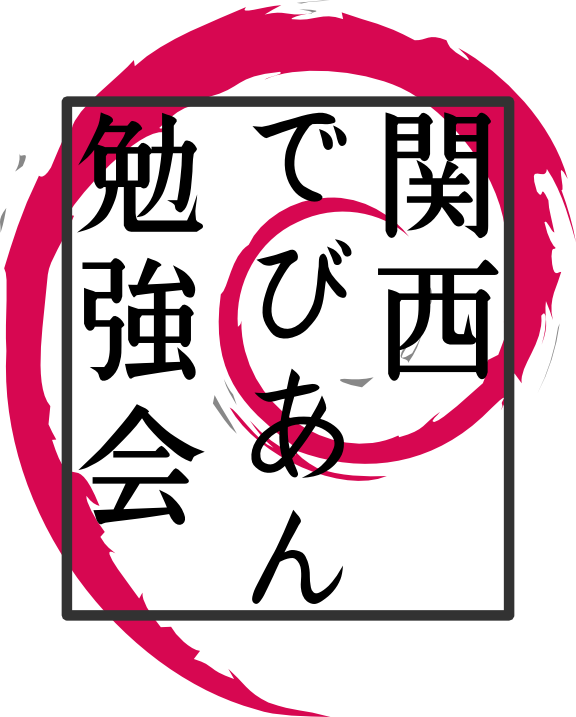
\includegraphics{image200802/kansaidebianlogo.png}
\end{center}

\begin{flushright}
\hfill{}関西 Debian 勉強会担当者 山下 尊也\\
\hfill{}\debmtgyear{}年\debmtgmonth{}月\debmtgdate{}日
\end{flushright}

\thispagestyle{empty}
\end{titlepage}

\dancersection{Introduction}{山下 尊也}
 
 関西 Debian 勉強会はDebian GNU/Linux のさまざ
 まなトピック(新しいパッケージ、Debian 特有の機能の仕組、Debian 界隈で起
 こった出来事、などなど)について話し合う会です。

 目的として次の三つを考えています。
 \begin{itemize}
  \item MLや掲示板ではなく、直接顔を合わせる事での情報交換の促進
  \item 定期的に集まれる場所
  \item 資料の作成
 \end{itemize}

 それでは、楽しい一時をお楽しみ下さい。

\newpage

\begin{minipage}[b]{0.2\hsize}
 {\rotatebox{90}{\fontsize{80}{80}
{\gt 関西デビアン勉強会}}}
\end{minipage}
\begin{minipage}[b]{0.8\hsize}
\hrule
\vspace{2mm}
\hrule
\setcounter{tocdepth}{1}
\tableofcontents
\vspace{2mm}
\hrule
\end{minipage}

\dancersection{最近のDebian関係のイベント報告}{山下 尊也}

\subsection{第17回 関西 Debian 勉強会}

\subsubsection{発表内容}

\begin{itemize}
 \item Debian Live に Ubiquity を移植できるか?
 \item Debian Mentors の紹介
 \item 10分でわかるDebianフリーソフトウェアガイドライン(DFSG)
\end{itemize}


「Debian Live に Ubiquity を移植できるか?」は、
Debianでは、廃止されたパッケージの利用などの
問題があり、簡単には出来ないと言う事になりましたが、
Ubiquityのようなものが live-helper にはないため、
今後も、live-helper の動きなどに注目したいと思います。

「Debian Mentors の紹介」については、初心者がパッケージなどを作成する際に
本家とは違い、初心者をある程度許してもらえる空間として紹介して頂きました。
これにより、私をはじめ多くの人が、最初の一歩を歩む事が出来たと思います。

「10分でわかるDebianフリーソフトウェアガイドライン(DFSG)」
では、木下さんが携帯電話を用いて、DFSGについて紹介して下さいました。
DFSGの内容にライセンスが関係するため、ライセンスについて
熱い議論がかわされました。

その後、急遽、佐々木さんに講師をして頂きました。

懇親会は、鳥料理が中心の南風で行いました。
懇親会の際に、なぜ東京エリア Debian 勉強会と関西 Debian 勉強会では、なぜ
\LaTeX を利用しているのか?
また、\LaTeX 以外のツールではダメなのか?などの議論がありました。
東京エリア Debian 勉強会は、11月に \LaTeX 合宿を行うようです。
関西では、12月に資料作成や、今年度のまとめなどを行いたいと
思っているので、そこで \LaTeX でのハンズオンをやりたいと考えています。

他にこんなツールでも資料作成出来るよ!!と言うのがあれば、
そのツールについても検討したいので、ぜひ12月の際に紹介して下さい。

%% sasaki
% 図, 表の番号にセクション入れる
\def\thefigure{\thesection.\arabic{figure}}
\def\thetable{\thesection.\arabic{table}}
\dancersection{はじめての CDBS}{佐々木 洋平}
\setcounter{figure}{0}
\setcounter{table}{0}

\subsection{はじめに}

CDBS -- {\bf C}ommon {\bf D}ebian {\bf B}uild {\bf S}ystem は,
debian/rules の共通部分を抽出し共有することで, 
debian/rules を簡潔かつ理解しやすくすることを目的としたツールです.
%
\cite{lenny CDBS doc} の Introduction によれば, 当初の開発動機は GNU
autoconf \& GNU automake を使用している Debian パッケージの重複した
debian/rules をなんとかしたい, だった様です:
\begin{quotation}
    The motivating factor for CDBS was originally that more and more
    programs today are created using GNU Autoconf configure scripts and
    GNU Automake, and as such they are all very similar to configure and
    build.  It was realized that a lot of duplicated code in everyone's
    debian/rules could be factored out. ...
\end{quotation}

今では CDBS はもっと汎用的になっており, 
autotools に限らず, Gnome, KDE, Python, Haskel など, 
様々なパッケージの作成に使用できるようになっています.
%
\cite{CDBS ギャラリ}によると, 
現時点で CDBS を使用しているソースパッケージは 1805 個, 
ソースパッケージ全体の $\sim 16 \%$ だそうです
\footnote{これ, 正しいですかね? }.

ドキュメントで上げられている CDBS の利点は以下の通りです%
\footnote{%
\cite{CDBS doc} の CDBS advantages の超訳です - -;)
}:
\begin{enumerate}
    \item 簡潔で, 可読性が高く, 効率的な debin/ruls を作成できる.
    \item debhelper と autotools の呼び出しを自動化することによって,
          繰り返し作業を気にする必要がなくなる.
    \item カスタマイズ性に限界が無いので,
          メンテナはパッケージ作成時のより重要な問題に集中できる.
    \item 提供されるクラスは十分にテストされており,
          よくある問題を回避するための汚い hack をする必要がない.
    \item 既存のパッケージを CDBS へ移行するのは容易である.
    \item 拡張性が高い.
\end{enumerate}
確かにそうなんですけれども, 
以下の例では逆に何をしているのかわからなくて不安になったりします:
\begin{commandline}
#!/usr/bin/make -f
                                
include /usr/share/cdbs/1/rules/debhelper.mk
include /usr/share/cdbs/1/class/autotools.mk
\end{commandline}

ここでは \cite{CDBS doc} の冒頭をざっくり解説してみようと思います.

\subsection{CDBS のディレクトリ構成\& ファイル群}

CDBS の実態は細分化された Makefile 群です.
実際に {\tt /usr/share/cdbs/} 以下を眺めてみましょう:
\begin{commandline}
% ls -aR /usr/share/cdbs
/usr/share/cdbs/:
./  ../  1/

/usr/share/cdbs/1:
./  ../  class/  rules/

/usr/share/cdbs/1/class:
./                  autotools-vars.mk  hbuild.mk         perlmodule-vars.mk
../                 autotools.mk       kde.mk            perlmodule.mk
ant-vars.mk         cmake.mk           langcore.mk       python-distutils.mk
ant.mk              docbookxml.mk      makefile-vars.mk  qmake.mk
autotools-files.mk  gnome.mk           makefile.mk

/usr/share/cdbs/1/rules:
./   buildcore.mk  debhelper.mk  patchsys-quilt.mk   tarball.mk
../  buildvars.mk  dpatch.mk     simple-patchsys.mk  utils.mk
\end{commandline}
中間ディレクトリ{\bf 1} は
将来の API 変更を考慮したディレクトリです.
rules, class ディレクトリ以下にあるファイルが
細分化された Makefile です.
パッケージを作成する際には
これらのファイルを適宜 debian/rules 内で include して使用します.
個々の Makefile の依存関係は以下の通りです:
%
\begin{figure}[htbp!]
 \begin{center}
  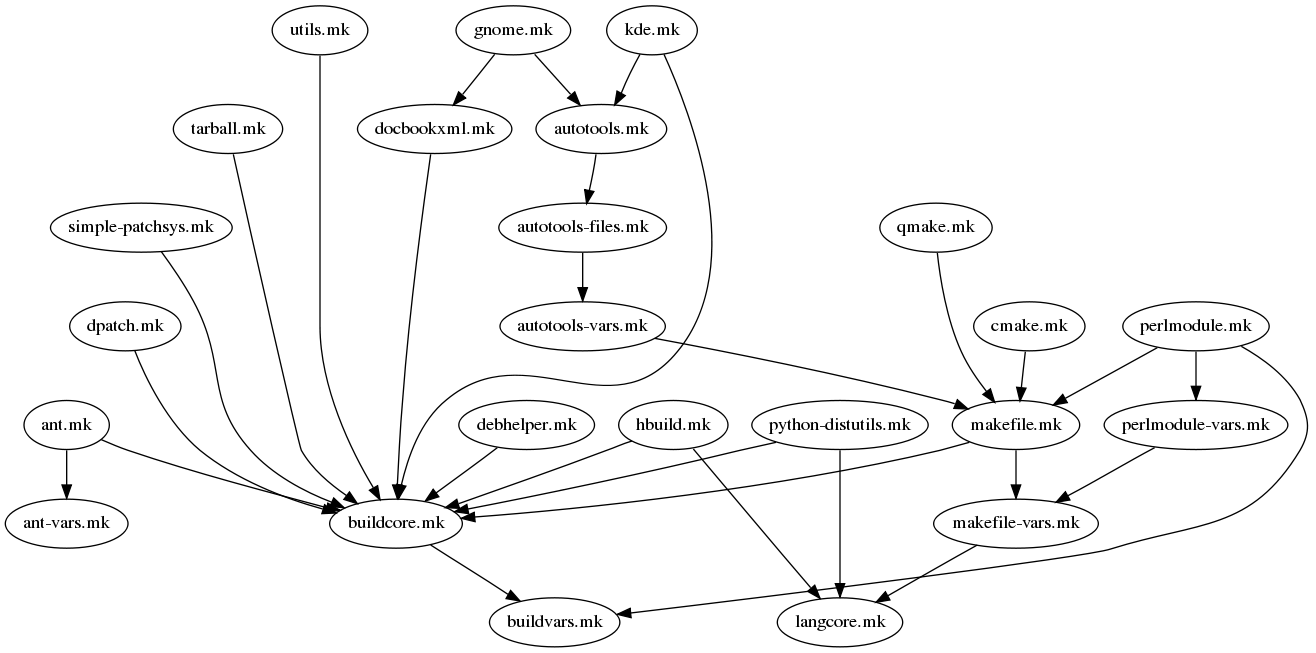
\includegraphics[width=160mm]{image200810/cdbs-mk-depend.png}
 \end{center}
    \caption{%
    CDBS で提供される Makefile の依存関係
    (\cite{lenny CDBS doc}).
    }
    \label{fig:cdbs-mk-depend}
\end{figure}

\subsection{基本となる rules}
\label{section:rules}

\subsubsection{buildvars.mk}

buildvars.mk を include すると
パッケージ作成のための環境変数が設定されます.
%
設定される変数の一覧を表 \ref{table:buildvars.mk} に記載します.
%
良く使われるのは {\tt CURDIR} と {\tt DEB\_DESTDIR} でしょう.
%
\begin{table}[htbp!]
    \begin{center}
        \caption{{\tt /usr/share/cdbs/1/rules/buildvars.mk} で設定される変数}
        \label{table:buildvars.mk}
        {\small 
        \begin{tabular}[tb]{|l|l|}
            \hline
            {\tt CURIDR} & 
            パッケージを作成しているディレクトリの名前.\\
            \hline
            {\tt DEB\_SOURCE\_PACKAGE} & 
                ソースパッケージの名前.\\
            \hline
            {\tt DEB\_VERSION} & 
                完全な Debian Version.\\
            \hline
            {\tt DEB\_NOEPOCH\_VERSION} & 
                Debian version without epoch .\\
            \hline
            {\tt DEB\_ISNATIVE} & 
                native パッケージの場合は空ではない(条件分岐に使用)..\\
            \hline
            {\tt DEB\_ALL\_PACKAGES} & 
                作成される全てのパッケージのリスト.\\
            \hline
            {\tt DEB\_INDEP\_PACKAGES} & 
                アーキテクチャに依存しないパッケージのリスト.\\
            \hline
            {\tt DEB\_ARCH\_PACKAGES} & 
                アーキテクチャに依存するパッケージのリスト.\\
            \hline
            {\tt DEB\_PACKAGES} & 
                通常の(udeb ではない)パッケージのリスト.\\
            \hline
            {\tt DEB\_UDEB\_PACKAGES} & 
                udeb の場合, そのリスト.\\
            \hline
            {\tt DEB\_ARCH} & 
                Debian アーキテクチャ. 後方互換のために残されている..\\
            \hline
            {\tt DEB\_HOST\_ARCH\_CPU} & 
                Debian アーキテクチャの CPU 情報.\\
            \hline
            {\tt DEB\_HOST\_ARCH\_OS} & 
                Debian アーキテクチャの OS 情報.\\
            \hline
            {\tt DEB\_DESTDIR} & 
                パッケージ作成の際にソフトを install するディレクトリ. .\\
            & 単一パッケージの場合, {\tt \$(CURDIR)debian/パッケージ名} \\
            & 複数のパッケージを作成する場合には {\tt \$(CURDIR)debian/tmp}\\
            \hline
        \end{tabular}
        }
    \end{center}
\end{table}
これらの変数を変更したい場合には, buildvars.mk を include した後で
debian/rules 内部で以下の様に設定します:
\begin{commandline}
# where sources are
DEB_SRCDIR = $(CURDIR)/src
# in which directory to build
DEB_BUILDDIR = $(DEB_SRCDIR)/build
# in which directory to install the sofware
DEB_DESTDIR = $(CURDIR)/destination
\end{commandline}

\subsubsection{buildcore.mk によるターゲットの設定}

buildcore.mk はパッケージ作成のための基本的なターゲットを提供します.
\cite{ポリシー}によれば, パッケージ作成の際
debian/rules ファイルの中で外部から参照されうるターゲットは,
以下の通りです:
\begin{itemize}
    \item build
    \item binary, binary-arch, binary-indep
    \item build-arch, build-indep (optional)
    \item get-orig-source (optional)
    \item clean (optional)
    \item path (optional)
\end{itemize}
buidcore.mk を include すると 
これらのターゲットが {\bf 細分化されて}提供されます.
buildcore.mk が提供する
ターゲットの一覧を図\ref{fig:cdbs-target}に示します.
%
\begin{figure}[htbp!]
 \begin{center}
  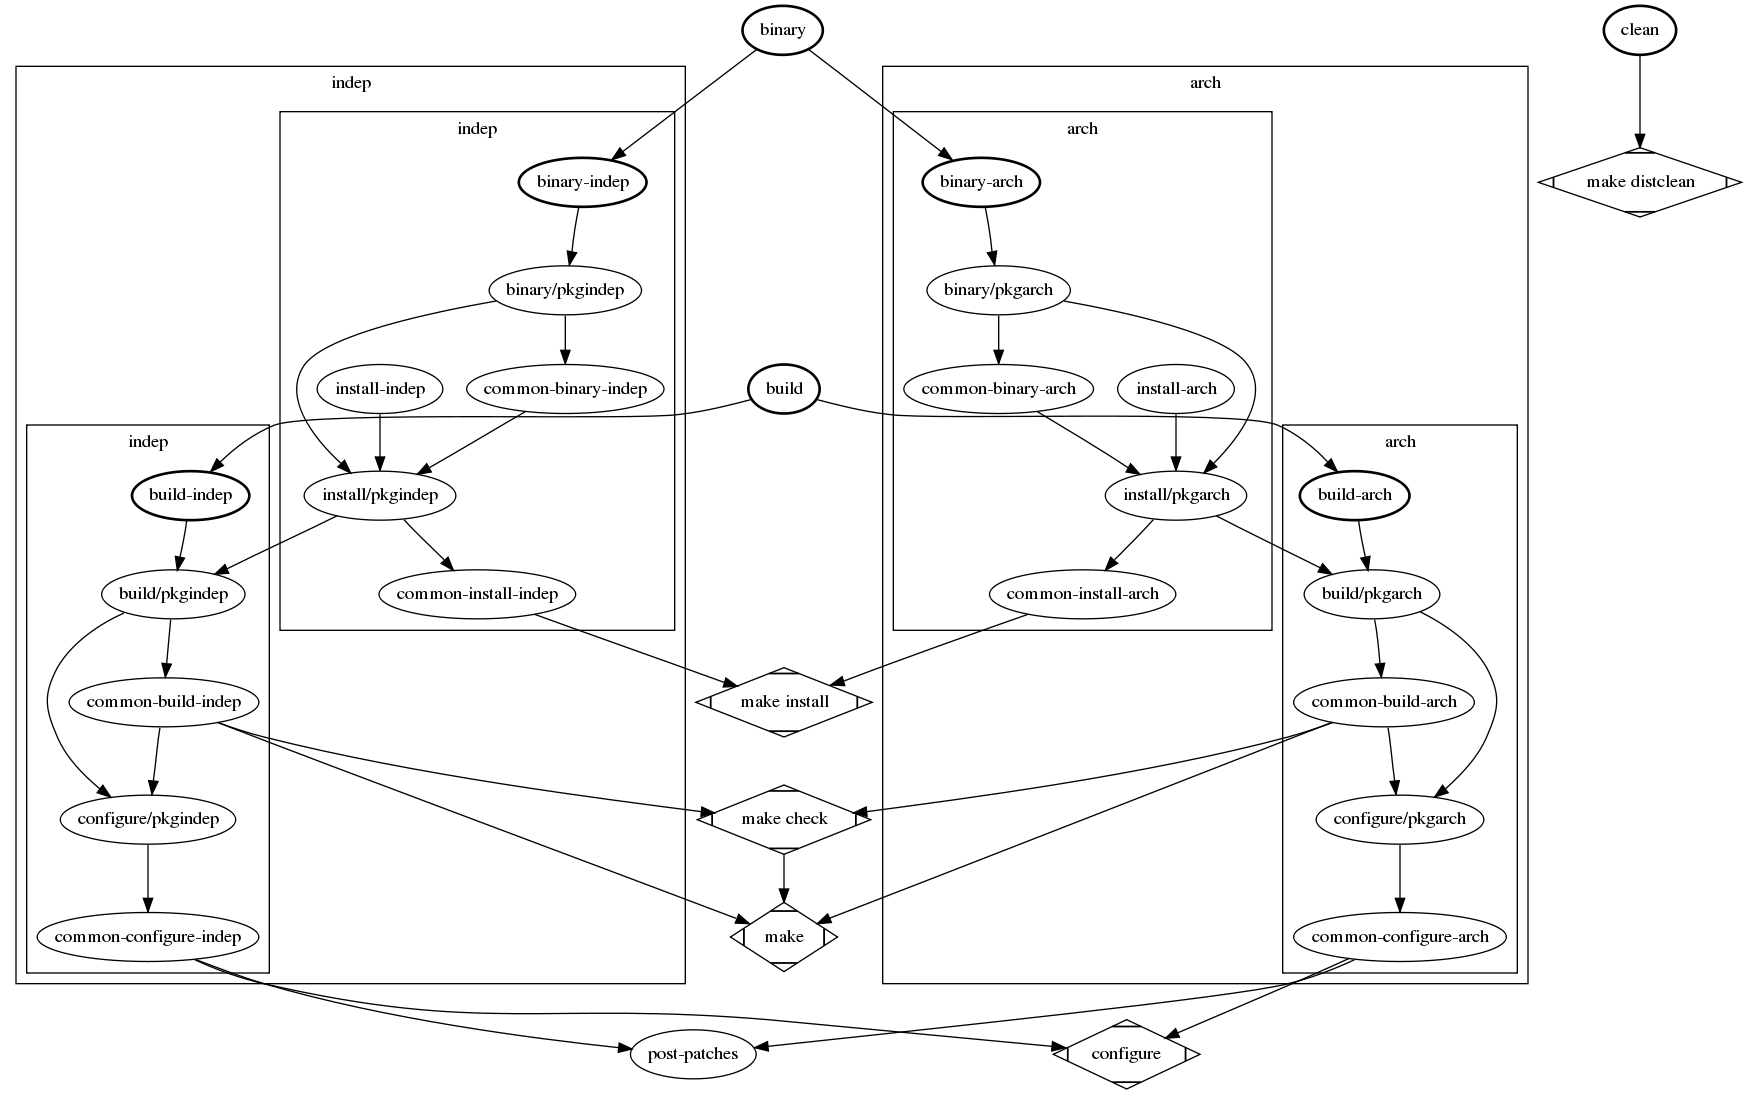
\includegraphics[width=160mm]{image200810/cdbs-target.png}
 \end{center}
    \caption{%
    buildcore.mk で提供されるターゲットの流れ
    (\cite{lenny CDBS doc}).
    }
    \label{fig:cdbs-target}
\end{figure}

実際には, buildcore.mk 自体はパッケージに対してなんの処理もしません. 
よって適宜 rules を記述することになります. 
例として, \cite{CDBS doc} に記載されている foo ついて解説します.
ここで foo は
\begin{itemize}
    \item ソースパッケージ foo を生成
    \item バイナリとして foo(arch-dep) と foo-data(arch-indep) を生成
\end{itemize}
するパッケージだとします.
\begin{commandline}
#!/usr/bin/make -f
include /usr/share/cdbs/1/rules/buildcore.mk

# pre-configure action
makebuilddir/foo::
        ln -s plop plop2
# post-configure action
configure/foo::
    sed -ri 's/PLOP/PLIP/' Makefile
configure/foo-data::
    touch src/z.xml
# post-build action
build/foo::
    /bin/bash debian/scripts/toto.sh
build/foo-data::
    $(MAKE) helpfiles
# post-install action
install/foo:
    cp debian/tmp/myfoocmd debian/foo/foocmd
      find debian/foo/ -name ``CVS'' -depth -exec rm -rf {} \;
install/foo-data:
    cp data/*.png debian/foo-data/usr/share/foo-data/images/
    dh_stuff -m ipot -f plop.bz3 debian/foo-data/libexec/
# post deb action
binary/foo:
    strip --remove-section=.comment --remove-section=.note --strip-unneeded \
      debian/foo/usr/lib/foo/totoz.so
# pre-clean action
cleanbuilddir/foo::
    rm -f debian/fooman.1
\end{commandline}
コメントとしてターゲットを記述するタイミングを記載しました.
ターゲットの記法は
\begin{center}
    {\tt {\bf target/packagename::}}
\end{center}
です. 後ろの {\tt {\bf ::}} が重要です.

\subsubsection{debhelper.mk による dh\_ の自動化}

CDBS の一番の御利益が, この debhelper.mk です.
CDBS では主な dh\_\* コマンドの呼び出しを debhelper.mk において行なうため,
debian/rules 内の dh\_\* の殆んどが不要になります.
debhelper.mk によって呼び出される dh\_\* を
表\ref{table:debhelper.mk}に示します.
\begin{table}[htbp!]
    \begin{center}
        \caption{%
        {\tt /usr/share/cdbs/1/rules/debhelper.mk} で管理される dh\_ コマンド}
        \label{table:debhelper.mk}
        \begin{tabular}[tb]{|llll|}
            \hline
            dh\_builddeb  & 
            dh\_installchangelogs  &
            dh\_installemacsen  & 
            dh\_installman   \\
            dh\_perl & 
                dh\_clean  & dh\_installcron  & dh\_installexamples \\
            dh\_installmenu  & 
                dh\_shlibdeps & dh\_compress  & dh\_installdeb  \\
            dh\_installinfo  & 
                dh\_installpam  & dh\_strip   & dh\_fixperms  \\
            dh\_installdebconf  & 
                dh\_installinit  & dh\_link  & dh\_gencontrol  \\
            dh\_installdirs  & 
                dh\_installlogcheck  & dh\_makeshlibs  & dh\_install  \\
             dh\_installdocs  & dh\_installlogrotate  & dh\_md5sums & \\
            \hline
        \end{tabular}
    \end{center}
\end{table}

debhelper.mk によって呼び出される dh\_ コマンドに対しては,
パラメータ設定は(大抵の場合)不要です. 
debelpher の呼び出しをカスタマイズする変数は 
debhelper.mk 冒頭のコメント行を参照して下さい.
\cite{CDBS doc} には以下の例があります:

\noindent {\bf 依存関係がシビアな共有ライブラリについて}
\begin{commandline}
DEB_DH_MAKESHLIBS_ARGS_libfoo := -V''libfoo (>= 0.1.2-3)``
DEB_SHLIBDEPS_LIBRARY_arkrpg := libfoo
DEB_SHLIBDEPS_INCLUDE_arkrpg := debian/libfoo/usr/lib/
\end{commandline}
\noindent {\bf ChangeLog のファイル名が一般的でない場合}
\begin{commandline}
DEB_INSTALL_CHANGELOGS_ALL := ProjectChanges.txt
\end{commandline}
\noindent {\bf .py を圧縮せずにパッケージ化する場合}
\begin{commandline}
DEB_COMPRESS_EXCLUDE := .py
\end{commandline}

ここでの記法
\begin{center}
    {\tt {\bf :=}}
\end{center}
に注意して下さい. 
{\tt {\bf :=}} は上書きです. 
CDBS の提供する変数に追加する場合には {\tt {\bf +=}} を使用します.

\subsubsection{patch の管理}

dpatch, quilt, そして CDBS 用の simple-patchsys の rules が提供されていま
す.  quilt, dpatch については include するだけで patch を適用する rule が
適用されます. 
%

simple-patchsys の場合は debian/patches に patch を置くだけ
で, パッケージ作成時に patch を適用し clean の際には元に戻します.
patch level は 3 まで ok です. 自動的に適用しようと試みます.

\subsection{class を使用する}

前小説で rules について簡単にまとめました. 
ここでは幾つかの class について紹介します.

\subsubsection{Makefile の場合:makefile.mk}

autotools を使わず Makefile のみを使用するソフトウェアには
makefile.mk が便利です. 
\cite{CDBS doc} では,
元々の Makefile が
\begin{itemize}
    \item 名前が MaKeFile で
    \item make mrproper で clean 
    \item make myprog で build
    \item make check  で check
    \item make install で install
\end{itemize}
というソフトウェアの場合について例示しています:
\begin{commandline}
#!/usr/bin/make -f
include /usr/share/cdbs/1/rules/debheper.mk
include /usr/share/cdbs/1/class/makefile.mk

DEB_MAKE_CLEAN_TARGET    := mrproper
DEB_MAKE_BUILD_TARGET    := myprog 
DEB_MAKE_INSTALL_TARGET  := install DESTDIR=$(CURDIR)/debian/tmp/
# no check for this software
DEB_MAKE_CHECK_TARGET    := check
# allow changing the makefile filename in case of emergency exotic practices
DEB_MAKE_MAKEFILE        := MaKeFiLe
# example when changing environnement variables is necessary :
DEB_MAKE_ENVVARS         := CFLAGS=''-fomit-frame-pointer''
\end{commandline}

\subsubsection{Autotoolsの場合: autotools.mk}

いわゆる {\tt configure \&\& make \&\& make install} なソフトウェアの場合は
autotools.mk が便利です. 
%
冒頭にも例示しましたが, 
標準的な autotools を使用するソフトウェアの場合には
\begin{commandline}
#!/usr/bin/make -f

include /usr/share/cdbs/1/rules/debheper.mk
include /usr/share/cdbs/1/class/autotools.mk
\end{commandline}
となります. 

configure へのオプションや環境変数の設定を行なう場合には
以下の様にします:
\begin{commandline}
DEB_CONFIGURE_EXTRA_FLAGS := --with-ipv6 --with-foo
COMMON_CONFIGURE_FLAGS := --program-dir=/usr
DEB_CONFIGURE_SCRIPT_ENV += LDFLAGS='' -Wl,-z,defs -Wl,-O1''
\end{commandline}
ここでも {\tt +=}, \tt{ :=} の意味は変わりません.
例えば
\begin{commandline}
#!/usr/bin/make -f

include /usr/share/cdbs/1/rules/debheper.mk
include /usr/share/cdbs/1/class/autotools.mk

# normally
DEB_MAKE_INSTALL_TARGET := install DESTDIR=$(DEB_DESTDIR)
# example to work around dirty makefile
# DEB_MAKE_INSTALL_TARGET := install prefix=$(CURDIR)/debian/tmp/usr
DEB_MAKE_CLEAN_TARGET := distclean
# example to activate check rule
DEB_MAKE_CHECK_TARGET := check
# overriding make-only environnement variables :
# (should never be necessary in a clean build system)
# (example borrowed from the bioapi package)
DEB_MAKE_ENVVARS    := ``SKIPCONFIG=true''
\end{commandline}
など.

他にも Perl, Python, Ruby, GNOME, KDE, Ant, HBuild(Haskel) 用の 
class があります

\subsection{まとまってないまとめ}

そんな所で時間が切れてしましました%
\footnote{数日前 HDD が逝って四苦八苦してました.うー}.

CDBS を使いはじめたら, もう debhelper には戻れない体になってしまうわけで
すが, いかんせん CDBS ってドキュメント少ないんですよね. 
%
この文書が最初の一歩になれば幸いです.

\newpage
\begin{thebibliography}{99}
    \bibitem[CDBS Documentation Rev. 0.4.0]{CDBS doc}
                    Marc (Duck) Dequ\'enes,
                    Arnaud (Rtp) Patard, 
                    2007:
                    CDBS Documentation,
                    \url{http://perso.duckcorp.org/duck/cdbs-doc/cdbs-doc.xhtml}
                    \newline
                    CDBS の online ドキュメンテーションです. 
                    パッケージに含まれているドキュメントより, 
                    こっちの方が情報が多く, 参考になります.
                    
    \bibitem[CDBS Documentation Rev.0.1.2]{lenny CDBS doc}
                    Marc (Duck) Dequ\'enes,
                    Arnaud (Rtp) Patard, 
                    Peter Eisentraut,
                    Colin Walters,
                    2007:
                    {\tt /usr/share/doc/cdbs/cdbs-doc.html}.
                    \newline
                    Lenny の CDBS(ver. 0.4.52) 付属のドキュメントです.
                    Web で公開されているドキュメントよりは古いです.

    \bibitem[CDBS 移行への 1st step]{CDBS 1st}
                    Tatsuki Sugiura, 2006:
                    CDBS 移行への 1st step
                    \url{http://sugi.nemui.org/doc/cdbs/cdbs-trans-1st.html}\\
                    既存のパッケージを CDBS へ移行する場合, 
                    非常に参考になると思います.

    \bibitem[Online CDBS Gallery]{CDBS ギャラリ}
                    Online CDBS Gallery, 
                    \url{http://cdbs.ueberalles.net/index.html}\\
                    CDBS を使っている debian/rules を見ることができます.
                    新たに CDBS へ移行する際に参考になるでしょう.
                    
    \bibitem[Debian Policy Manual]{ポリシー}
                    Ian Jackson \& Christian Schwarz, 1996:
                    Debian Policy Manual,
                    \url{http://www.debian.org/doc/debian-policy/}

    \bibitem[Debian パッケージ作成の手引き]{パッケージ手引き}
                    小林 儀匡, 
                    Debianパッケージ作成の手引き,
                    \url{http://www.debian.or.jp/~nori/debian-packaging-guide/index.html}
                    \newline
                    Debian パッケージ作成の手引きです.
                    「debhelper を使わない場合 → 
                    使う場合 →
                    CDBS への移行」と順序立てて説明されています.

    \bibitem[やまだ \& 鵜飼(2006)]{入門 Debian パッケージ}
                    やまだあきら(著), 鵜飼文敏(監修), 2006:
                    入門 Debian パッケージ, 技術評論社,
                    ISBN4-7741-2768-X
\end{thebibliography}
\setcounter{figure}{0}
\setcounter{table}{0}

%% araki
\dancersection{cdn.debian.or.jp, cdn.debian.netにおける取り組み}{荒木 靖宏}

いつでも必要なソフトウェアやコンテンツを安価に入手する手段としてCDNが広
くつかわれている。 Debianはdebの安定入手手段の有無がシステム の信頼性を
左右するシステムであり、その特殊性を考慮したCDNシステムが必要となる。 今
回はcdn.debian.or.jp, cdn.debian.netにおける取り組みを紹介する。

\subsection{CDNとは}

Content Delivery Network(CDN)はウェブコンテンツ配置および配送方法とし
てAkamai社によりサービスされ広く知られることになった。当初から一部の人気
の高いサーバへのトラフィック集中によるサーバ停止の回避、海外のリッチコン
テンツ取得の高速化、トラフィック分散によるネットワークおよびサーバの利用
平準化などの理由で広く受け入れられた。

CDNという用語自体はWWWに限ることなく、一般にコンテンツを取得するための配
送手段や方法全体を指す場合がある。たとえば、WinnyやBittorrentなどのコン
テンツを取得するために特別に設計されたプロトコルを用いて、P2Pネットワー
クを構成するような手法も含まれる。

\subsection{DebianにおけるCDNの現状}

\subsubsection{利用法とユーザから見た動作}

cdn.debian.or.jpではDebianでインストール時から広くdebファイルの入手に使
われるaptで使えるCDNとして設計し、運用している。そのため、Debianにおける
CDNの利用法は至極簡単である。/etc/apt/source.listに記述するAPTリポジトリ
として、

\begin{commandline}
deb http://cdn.debian.or.jp/debian/ stable main contrib non-free
deb-src http://cdn.debian.or.jp/debian/ stable main contrib non-free
\end{commandline}

以上のように指定するだけでユーザは今までとなんら変わることなくaptコマン
ドを使用できる。

現在、cdn.debian.or.jp, ftp.jp.debian.org, cdn.debian.netの名で運用して
いる。

\begin{figure}[htbp]
 \begin{center}
  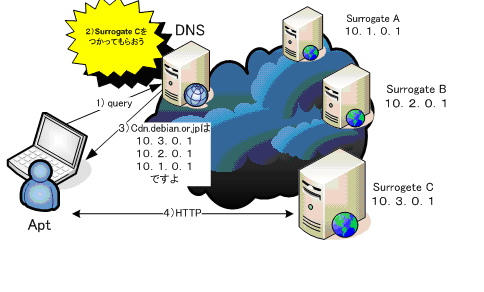
\includegraphics[width=100mm]{image200810/cdn-userviwer.png}
 \end{center}
 \caption{ユーザから見た cdn.debian.or.jp の動作}
 \label{fig:cdn-userviwer}
\end{figure}

サービス時の手順と構成は以下のようになる。(図\ref{fig:cdn-userviwer})

\begin{enumerate}
 \item ユーザがapt-getコマンドを行うとcdn.debian.or.jpをDNSで問い合わせ
       る
 \item cdn.debian.or.jpを管理するDNSはサーバ候補(surrogate)選択する
 \item 選択結果をDNSのリプライとして返す
 \item aptはcdn.debian.or.jpとしてSurrogate Cを使用する。
\end{enumerate}

\subsubsection{構築の方法}

実際にはクライアントDNSは次のように動作している。

\begin{enumerate}
 \item クライアントDNSがcdn.debian.or.jpを検索すると、CNAME
       deb.cdn.araki.netがdebian.or.jpのDNS(BIND)から返答される。
 \item クライアントDNSはdeb.cdn.araki.netを得るためにcdn.araki.netのNSレ
       コードを問い合わせて、ns.cdn.araki.net, plat.debian.or.jp,
       debian.topstudio.co.jp, osdn2.debian.or.jpを得る。
 \item クライアントDNSはいずれかのホストにdeb.cdn.araki.netのAレコードを
       問い合わせて、サロゲートのIPアドレスをdns\_balanceから得る。
 \item クライアントDNSは、ユーザクライアントに3で得た情報を返す。
\end{enumerate}

2を実現するためのAraki.netのBIND設定は次のようになる。

\begin{commandline}
cdn             IN      NS      ns.cdn
                IN      NS      plat.debian.or.jp.
                IN      NS      debian.topstudio.co.jp.
                IN      NS      osdn2.debian.or.jp.
\end{commandline}

\textit{DNS Balance はユーザのIPアドレスと、何らかの方法でサーバをランク
づけした表を元にユーザが接続すべきサイトを指示します。この表は一定時間毎
に読み込み直され、これにより動的な負荷分散が可能です。}

(DNS Balanceの配布ページ\url{http://www.dnsbalance.ring.gr.jp}より)

3を実現するためのdns\_balanceの設定は次のようなサーバをランク付けしたruby
形式のファイルである。

\begin{commandline}
$addr_db = {
  "default" => {
    "ns.cdn.araki.net" => [
      [[210,157,158,38], 0],
    ],
    "localhost" => [
      [[127,0,0,1], 0],
    ],
 "deb.cdn.araki.net" => [
                [[61,115,118,67], 1000],
                [[133,50,218,117], 10],
                [[202,229,186,27], 20],
                [[133,5,166,3], 10],
                [[130,54,59,159], 10],
                [[210,157,158,38], 9900],
        ], },}
\end{commandline}

この設定ファイルに基づき、ホストIPアドレスの後ろの数字は優先度であり、
1(優先度高)から9999(優先度最低)までの整数で指定する。

\subsubsection{cdn.debian.or.jpのシステムと動作}

CDNシステムが完全に動作しユーザから使用されるためには、システムが完全な
ファイルを提供すること、システムが安定して動作すること、そしてCDNを使っ
た場合に高速に動作していることが求められる。

\subsubsubsection{提供ファイルの完全性}

このために以下二点を満たさねばならない。

\begin{itemize}
 \item 個々のファイルがコンテンツ提供者たるdebファイル配布元と同一である
       こと
 \item apt-get updateの結果取得するファイル群がどのSurrogateでも入手でき
       ること
\end{itemize}

前者については、debはそのファイルのmd5値、sha1値とともに配布され、ユーザ
が使用するaptで確認後に利用されるためCDNを使用した場合でも問題にならない。

後者についてはユーザがapt-get updateを行ったときに接続するSurrogateと
apt-get dist-upgradeを行ったときに接続するSurrogateは同一であるとは限ら
ないため、DNSがSurrogateとして返すサーバが保持するファイルは同一である必
要がある。cdn.debian.or.jpではDebianプロジェクトで一般に行われている方法
と同様に、rsyncプロトコルを用い、pushミラーを行っている(図\ref{fig:cdn-rsync})。そのた
め、cdn.debian.or.jpのサロゲート内で最上流にあるサーバとミラーが同一であ
ることを2分毎にrsyncミラー終了時に作成されるスタンプファイルを確認して、
同一でないサーバはサロゲート候補から一時的に除外している。

ただし、これはミラーの配送ツリーの管理を行う必要があるため、日本国内のミ
ラーに限定している。

\begin{figure}[htbp]
 \begin{center}
  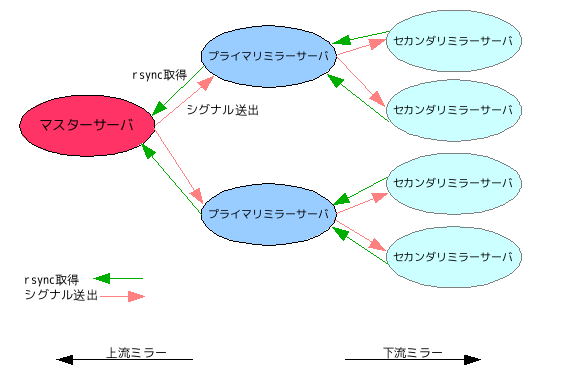
\includegraphics[width=100mm]{image200810/cdn-rsync.png}
 \end{center}
 \caption{Debianサロゲートのrsyncによるミラー}
 \label{fig:cdn-rsync}
\end{figure}

\subsubsubsection{システムの安定動作}

先に述べたように、ユーザはCDNを使用する際にはDNSを最初に使用するため、
DNSの安定運用がカギとなる。そのため、cdn.debian.or.jpを管理するDNSサーバ
はまったく独立に動作するサーバで行っている。

また、サーバの動作を確認は、5秒以内にHTTPのレスポンスを返さないサーバは
サロゲート候補から一時的に除外している。

後述するように、サロゲートの生死確認は2分ごとにdns\_balanceの動作に反映さ
れる。ローカルDNSにキャッシュされる情報とあわせて最悪でも3分以内に動作し
ていないサーバは排除される。

\newpage

\subsubsubsection{高速動作}

cdn.debian.or.jpではDNSで問い合わせされるとサロゲートリストとして複数の
IPアドレスを返す。このIPアドレスはラウンドロビンで選択しているわけではな
く、提供可能なサーバキャパシティやネットワーク速度を考慮し、設定している。

\subsubsection{IPアドレスの位置情報を使用したサーバ選択}

当初はcdn.debian.or.jpとして運用していたものの、その後にglobalに分散する
Debianミラーに対応させた。

globalにCDNを展開する場合には地理的に近いサーバ群からある程度絞込むのが
有効である。現在、GeoIPなど無料でIPと地理情報のマッピング提供者が現れて
おり、debianパッケージになっていることもあり、本システムではMaxmindの
GeoIPを使用している。

Dns\_balanceにはASあるいはネットワークアドレスごとに振り分けるIPアドレス
の指定が可能であるが、

\begin{itemize}
 \item Debianのミラーは国別地域別に制御されていること
 \item 16ビットで指定されるASとAS間の経路の測定が難しい
 \item 個々のネットワーク間の経路を指定するのは現実的でない
\end{itemize}

以上の理由から、dns\_balanceに接続するIPアドレスの国名、大陸名を逆引きし、
その結果をつかって返すAレコードを変更するようにdns\_balanceを拡張してい
る。

大陸別の設定ファイルは次のように、6大陸別である。

\begin{commandline}
yaar@loon3:~/playground/cdn$ ls continent/
AF_deb_cdn_araki_net.rb  EU_deb_cdn_araki_net.rb  OC_deb_cdn_araki_net.rb
AS_deb_cdn_araki_net.rb  NA_deb_cdn_araki_net.rb  SA_deb_cdn_araki_net.rb
\end{commandline}

さらに国別の設定ファイルを置く。

\begin{commandline}
yaar@loon3:~/playground/cdn$ ls country/
FRA_deb_cdn_araki_net.rb  JPN_jp_cdn_araki_net.rb
JPN_deb_cdn_araki_net.rb  KOR_deb_cdn_araki_net.rb
\end{commandline}

これらの設定ファイルをつかって、dns\_balanceが実際に読み込む次のような設
定ファイルを2分ごとに作成している。サーバの生死確認などはこのタイミング
で反映される。

\begin{commandline}
$addr_db = {"default"=>{"localhost"=>[[[127, 0, 0, 1], 0]], "deb.cdn.araki.net"=
>[[[61, 115, 118, 67], 1000], [[61, 206, 119, 174], 20], [[202, 229, 186, 27], 2
0], [[203, 178, 137, 175], 9000], [[210, 157, 158, 38], 9900]], "ns.cdn.araki.ne
t"=>[[[210, 157, 158, 38], 0]], "jp.cdn.araki.net"=>[[[61, 115, 118, 67], 1000],
 [[61, 206, 119, 174], 20], [[202, 229, 186, 27], 20], [[203, 178, 137, 175], 90
00], [[210, 157, 158, 38], 9900]]}, "KOR"=>{"deb.cdn.araki.net"=>[[[143, 248, 23
4, 110], 20]]}, "SA"=>{"deb.cdn.araki.net"=>[]}, "EU"=>{"deb.cdn.araki.net"=>[[[
141, 76, 2, 4], 9000]]}, "AF"=>{"deb.cdn.araki.net"=>[]}, "AS"=>{"deb.cdn.araki.
net"=>[[[61, 115, 118, 67], 1000], [[61, 206, 119, 174], 20], [[202, 229, 186, 2
7], 20], [[203, 178, 137, 175], 9000], [[210, 157, 158, 38], 9900]]}, "JPN"=>{"d
eb.cdn.araki.net"=>[[[61, 115, 118, 67], 1000], [[61, 206, 119, 174], 20], [[202
, 229, 186, 27], 50], [[203, 178, 137, 175], 9000], [[210, 157, 158, 38], 9900]]
, "jp.cdn.araki.net"=>[[[61, 115, 118, 67], 1000], [[61, 206, 119, 174], 20], [[
202, 229, 186, 27], 50], [[203, 178, 137, 175], 9000], [[210, 157, 158, 38], 990
0]]}, "NA"=>{"deb.cdn.araki.net"=>[[[204, 152, 191, 39], 9000], [[128, 30, 2, 36
], 9000], [[35, 9, 37, 225], 9000]]}, "OC"=>{"deb.cdn.araki.net"=>[[[150, 203, 1
64, 37], 9000]]}, "FRA"=>{"deb.cdn.araki.net"=>[[[193, 54, 19, 19], 9000], [[194
, 2, 0, 36], 9000]]}}
\end{commandline}

\newpage

\subsection{使用実績}

以下3ヶ月分のplat.debian.or.jpで動作しているDNSへのアクセス実績を示す。

\begin{itemize}
 \item 2008年7月16日から10月15日までの三ヶ月間の利用実績を解析した。
 \item 本システムではDNSのAまたはAnyに対して返答を戻すことから、それ以外
       のクエリに関しては無効なアクセスとして処理している。
 \item 地域はアクセス元のIPアドレスをGeoIPライブラリから算出している。
 \item 全DNS動作ホストは、plat.debian.or.jp, osdn2.debian.or.jp,
       debian.topstudio.co.jpであり、この3倍のクライアントからのアクセス
       があると推測される。
\end{itemize}

\begin{figure}[!h]
 \begin{tabular}{cc}
  \begin{minipage}{0.5\hsize}
   \begin{center}
    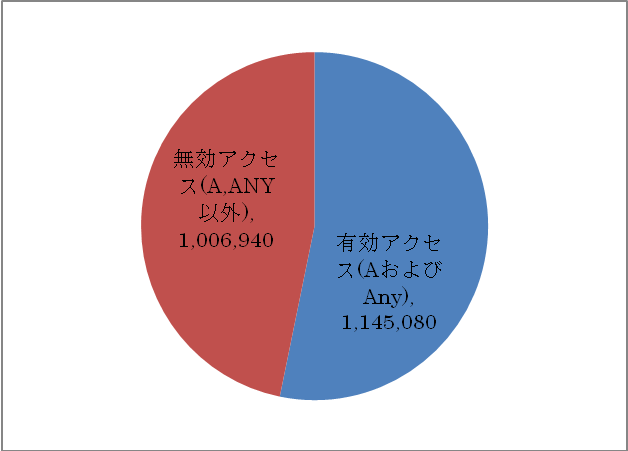
\includegraphics[width=0.7\hsize]{image200810/cdn-access.png}
    \caption{DNSアクセス種別}
    \label{fig:cdn-access}
   \end{center}
  \end{minipage}
  \begin{minipage}{0.5\hsize}
    \begin{center}
     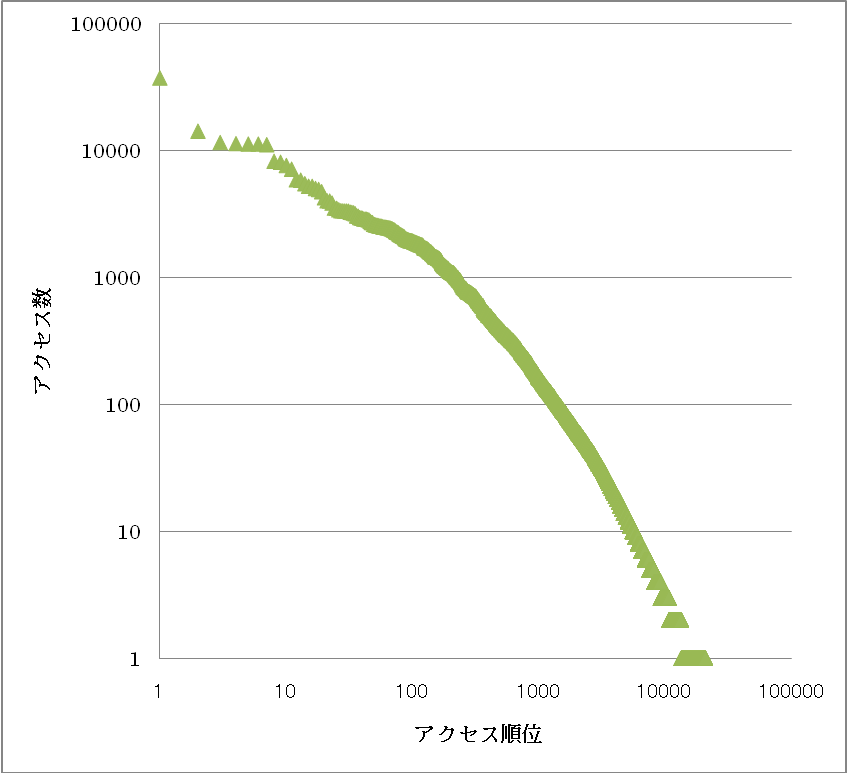
\includegraphics[width=\hsize]{image200810/cdn-access-rank.png}
     \caption{ホスト別アクセス順位とアクセス数}
     \label{fig:cdn-access-rank}
    \end{center}
  \end{minipage}
 \end{tabular}
\end{figure}

ユニークホスト数は20554であるが、その分布は極端に偏っている。

\newpage

\begin{figure}[!h]
 \begin{tabular}{cc}
  \begin{minipage}{0.3\hsize}
   \begin{center}
    \caption{DNSクエリ数上位20カ国}
    \begin{tabular}{|l|r|}
     \hline
     JPN & 808138 \\ \hline
     USA & 87767 \\ \hline
     CAN & 82566 \\ \hline
     KOR & 38596 \\ \hline
     CHIN & 26670 \\ \hline
     FIN & 14558 \\ \hline
     TWIN & 12527 \\ \hline
     IND & 7941 \\ \hline
     IDN & 6463 \\ \hline
     HKG & 5616 \\ \hline
     RUS & 3975 \\ \hline
     SGP & 3656 \\ \hline
     DEU & 2990 \\ \hline
     GBR & 2792 \\ \hline
     AUS & 2635 \\ \hline
     ESP & 2632 \\ \hline
     THA & 2623 \\ \hline
     MYS & 2475 \\ \hline
     PHL & 2359 \\ \hline
     ITA & 2196 \\ \hline
    \end{tabular}
    \label{dnsquerytop20}
   \end{center}
  \end{minipage}
  \begin{minipage}{0.7\hsize}
  \begin{center}
   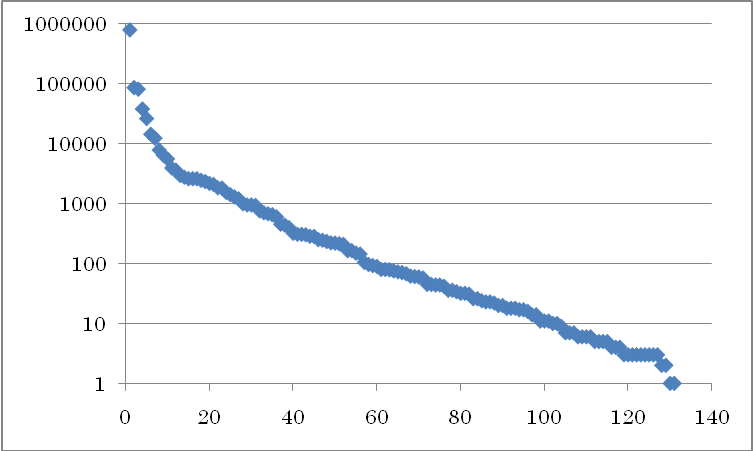
\includegraphics[width=\hsize]{image200810/cdn-query-topcountry.png}
   \caption{DNSクエリ数上位国(横軸)-クエリ数(縦軸)}
   \label{fig:cdn-query-topcountry}
  \end{center}
  \end{minipage}
 \end{tabular}
\end{figure}

なお、国が判定できないのは1552件、率にして0.135\%であった。

\begin{figure}[!h]
 \begin{tabular}{cc}
  \begin{minipage}{0.5\hsize}
   \begin{center}
    \caption{CDN振り分け先実績}
    \begin{tabular}{|l|r|l|}
     \hline
     地域 & \multicolumn{1}{l|}{アクセス数} &  \\ \hline
     アジア & 570137 &  \\ \hline
     アジア(日本と韓国除く) & \multicolumn{1}{l|}{} & \multicolumn{1}{r|}{55539} \\ \hline
     日本 & \multicolumn{1}{l|}{} & \multicolumn{1}{r|}{509367} \\ \hline
     韓国 & \multicolumn{1}{l|}{} & \multicolumn{1}{r|}{5231} \\ \hline
     ヨーロッパ & 16804 &  \\ \hline
     ヨーロッパ(フランス除く) & \multicolumn{1}{l|}{} & \multicolumn{1}{r|}{15154} \\ \hline
     フランス & \multicolumn{1}{l|}{} & \multicolumn{1}{r|}{1650} \\ \hline
     北米 & 142207 &  \\ \hline
     オセアニア & 10766 &  \\ \hline
     アフリカ & 160 &  \\ \hline
     その他 & 404996 &  \\ \hline
     総有効アクセス数 & 1145070 &  \\ \hline
    \end{tabular}
    \label{dnsquery}
   \end{center}
  \end{minipage}
  \begin{minipage}{0.5\hsize}
   \begin{center}
    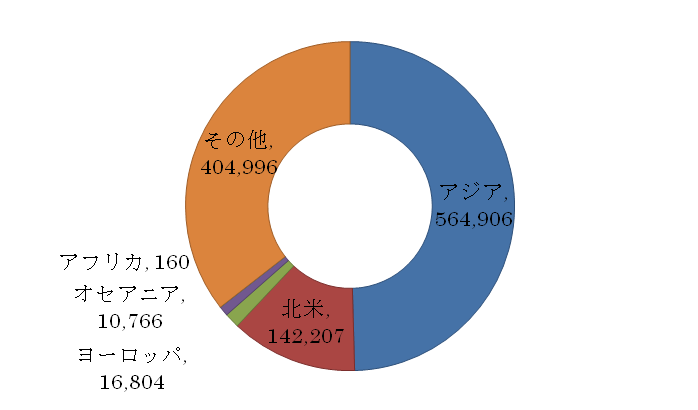
\includegraphics[width=0.9\hsize]{image200810/cdn-area-world.png}
    \caption{地域別振り分け実績}
    \label{fig:cdn-area-world}
   \end{center}
  \end{minipage}
 \end{tabular}
\end{figure}

\newpage

\begin{figure}[!h]
 \begin{tabular}{cc}
  \begin{minipage}{0.3\hsize}
   \begin{center}
    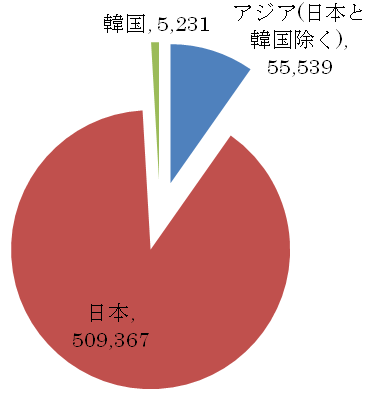
\includegraphics[width=0.8\hsize]{image200810/cdn-area-asia.png}
    \caption{アジア地域の振り分け実績}
    \label{fig:cdn-area-asia}
   \end{center}
  \end{minipage}
  \begin{minipage}{0.7\hsize}
   \begin{center}
    \caption{日本での振り分け実績}
    \begin{tabular}{|l|l|r|}
     \hline
     \textbf{ホスト名} & \textbf{IP} & \multicolumn{1}{l|}{\textbf{振り分け数}} \\ \hline
     runner.oyu-net.jp. & 61.206.119.174 & 690596 \\ \hline
     dwarf.topstudio.co.jp. & 202.229.186.27 & 660091 \\ \hline
     hanzubin.st.wakwak.ne.jp & 61.115.118.67 & 649512 \\ \hline
     studenno.kugi.kyoto-u.ac.jp. & 130.54.59.159 & 599550 \\ \hline
     dennou-q.geo.kyushu-u.ac.jp & 133.5.166.3 & 468730 \\ \hline
     frost.nemui.org. & 218.219.152.77 & 445589 \\ \hline
     dennou-h.ep.sci.hokudai.ac.jp. & 133.87.45.30 & 379888 \\ \hline
     ftp.nara.wide.ad.jp & 203.178.137.175 & 58825 \\ \hline
     plat.debian.or.jp & 210.157.158.38 & 6095 \\ \hline
    \end{tabular} 
   \end{center}
   \label{dnsjapansymmetry}
  \end{minipage}
 \end{tabular}
\end{figure}

% \begin{figure}[!h]
%  \begin{center}
%   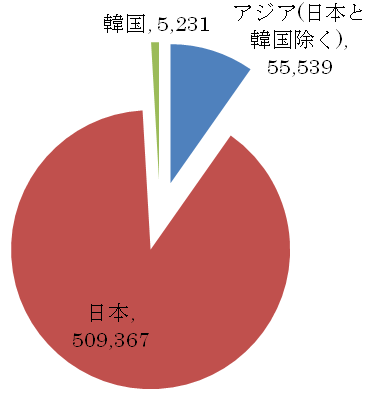
\includegraphics[width=100mm]{image200810/cdn-area-asia.png}
%  \end{center}
%  \caption{アジア地域の振り分け実績}
%  \label{fig:cdn-area-asia}
% \end{figure}

アジア地域向けのサーバおよび韓国地域向けのサーバは日本向けのサーバ群設定
と全く同一のものを設定している。

% \begin{table}[!h]
%   \caption{日本での振り分け実績}
%  \begin{center}
%   \begin{tabular}{|l|l|r|}
%    \hline
%    \textbf{ホスト名} & \textbf{IP} & \multicolumn{1}{l|}{\textbf{振り分け数}} \\ \hline
%    runner.oyu-net.jp. & 61.206.119.174 & 690596 \\ \hline
%    dwarf.topstudio.co.jp. & 202.229.186.27 & 660091 \\ \hline
%    hanzubin.st.wakwak.ne.jp & 61.115.118.67 & 649512 \\ \hline
%    studenno.kugi.kyoto-u.ac.jp. & 130.54.59.159 & 599550 \\ \hline
%    dennou-q.geo.kyushu-u.ac.jp & 133.5.166.3 & 468730 \\ \hline
%    frost.nemui.org. & 218.219.152.77 & 445589 \\ \hline
%    dennou-h.ep.sci.hokudai.ac.jp. & 133.87.45.30 & 379888 \\ \hline
%    ftp.nara.wide.ad.jp & 203.178.137.175 & 58825 \\ \hline
%    plat.debian.or.jp & 210.157.158.38 & 6095 \\ \hline
%   \end{tabular} 
%  \end{center}
%  \label{dnsjapansymmetry}
% \end{table}

日本での振り分け実績は、設定した頻度情報をほぼ正確に反映しており、プログ
ラムの動作および、期間中の各サロゲートに大きな障害がなかったことを示して
いる。

\subsection{関連研究とディスカッション}

\url{http://prisms.cs.umass.edu/~kevinfu/papers/secureupdates-hotsec06.pdf}
でのサーベイ結果のように、パッケージ配布にはいくつかの方法と危険性が指摘
されている。このサーベイ結果で指摘されるように、Debianでは個々のファイル
ごとにsha-1およびMD5,SHA-256のハッシュ値を配布している。

加えて、本システムの日本での運用においては、マスターサーバからサロゲート
へのファイル同期時に配送ツリーの確認とファイルの一致を確認しており、障害
時の排除機能を有するため、単なるファイルのミラーリング以上の安全性は確保
されている。


OpenSuse における配送
(mirrobrain, \url{http://en.opensuse.org/Build_Service/Redirector} )
はsourceforgeをはじめ多くのCDNで採用している方法である。クライアントへの
サロゲート決定の方法はGeoIPの使用しており、本システムと同等のものである。

ただし、Debianのaptシステムの制限により、本システムではHTTPリダイレクト
ではなく、DNSを使用している。

また、mirrorbrainではサロゲートへの配送の確認は行っていないものと思われ
る。


aptのP2P対応も有力な配布手段である。apt-p2p
(\url{http://www.camrdale.org/apt-p2p/})
により、aptのP2P対応が進められている。有力な候補である。ただし、Kashimir
プロトコルをクライアントで直接使うものであり、ネットワーク利用ポリシーと
の競合やinstall時に利用できない点、取得希望ファイルが入手できない場合に
HTTPにフォールバックするため速度に問題があり、今後検証すべき問題も多い。

サロゲートが正しく動作しているのか、その能力に応じたサロゲート使用ができ
ているかどうかは、分散したファイルサーバからのファイル入手において重要な
要素である。この組み合わせを考えると、表\ref{health check}のように分類される。本システ
ムでは、サーバやサーバとクライアント間のネットワークの実測を行わないこと、
ここのサロゲートの運用は独立して行うことでサロゲートへ特別なプログラムを
必要としないことで、コストの劇的な削減を可能としている。

\begin{table}[htbp]
\caption{}
\begin{tabular}{|l|l|l|}
\hline
 & 申告ベースの能力 & 動的測定・実績ベースの能力 \\ \hline
申告ベースのヘルスチェック & Debianミラーサーバリスト & Debianミラーの口コミ・トライアンドエラー \\ \hline
動的測定・実績ベースのヘルスチェック & 本システム & 理想的なシステムだがコスト大
商用CDNなど \\ \hline
\end{tabular}
\label{health check}
\end{table}

\subsection{課題と将来の展望}

ここまで説明してきた、cdn.debian.or.jpの動作には改善すべき点が多数存在する。改善の展望としていくつか挙げる。

\subsubsection{アクセス実績あるいはローカルポリシーに基いたCDN配置}

アクセス実績によると、日本、米国、カナダ、韓国、中国、フィンランド、台湾、
インド、インドネシア、ホンコン、ロシアと続く。現状では、大陸毎に設定され
たサロゲートは存在するものの、日本、韓国、アメリカを除けば各国毎に設定さ
れたサロゲートは存在しない。

このアクセス実績にもとづき、これらの国内のミラーを生かした設定を近い将来
行いたい。

\subsubsubsection{apt-getコマンドのHTTP REDIRECT}

apt-getコマンドはHTTP REDIRECTに対応していない。

そのため、前述したようにmirrorbrainなどのCDNは使用することができない。

HTTP REDIRECTは、いったんHTTP GETなどで接続してきたクライアントに対して、
新たにそのリソースが存在するURLを通知するものである。この仕組みをうまく
つかったCDNとして、Coral Content Distribution Network (Coral CDN)がある。
Coral CDNはサロゲート間でP2Pによるファイル配置し、そのインターフェースと
して、HTTPを使用し、しかも使用にはインターネットから取得可能なファイルで
あれば制限をかけていない。さらに、Apacheを使った一時配布サーバではHTTP
REDIRECTをつかってCoral CDNに誘導することも推奨されている。ただし、現状
で、Coral CDNを使うために、

\begin{commandline}
deb http://cdn.debian.or.jp.nyud.net:8090/debian/ stable main contrib non-free
\end{commandline}

を指定することも可能だが、少なくとも日本においてはCoral CDNを担うサロゲー
トが存在しないこともあって非常に低速である。ただし韓国や中国では広くつか
われており、将来の拡張に使用したい。

\subsubsubsection{マスターサーバからサロゲートへのミラーリング方法}

本システムでは既存のrsyncによるミラーリング手法には手をつけていない。行っ
たのはrsyncをつかってタイムスタンプを確認し、サロゲートのヘルスチェック
のひとつに使用したのみである。debianにおけるrsyncの使い方現状のミラーリ
ングに由来する問題は

\begin{enumerate}
 \item master.debian.orgからの末端までのあいだは冗長化されていない
 \item rsyncはディレクトリの同期を取る方法であり、ファイルの転送に必ずし
       も適していない。debのように依存関係を記述したメタデータを含むファ
       イルであれば、ファイル毎のpushであっても配送に問題はない
 \item 配送がユニキャストである
 \item 利用頻度や重要度にかかわらず同様の配送を行っている 
\end{enumerate}

等さまざまである。

Debianが潤沢なネットワーク環境と強力なCPUを要するホストでない場合でもミ
ラーリングないしサロゲートからのファイル入手を可能とするFLUTEなどの配送
手法が必要になろう。

\newpage 

\subsection{おわりに}

いつでも必要なソフトウェアやコンテンツを安価に入手する手段としてCDNはこ
れからも様々な発展を続けると考える。Debianはdebの安定入手手段の有無がシ
ステムの信頼性を左右するシステムであり、CDNの広範な活用が今後ますます求
められるようになると考える。

本システムの導入により、サロゲート個々の安定性がクライアントに直接影響す
ることはかなり抑えることができるが、より確実なパッケージ入手のために、信
頼性が高く安定動作しているサロゲートの増加をDebianプロジェクトでは引き続
き求めている。

\dancersection{今後の予定}{山下 尊也}

\subsection{次回}
次回は、2008年11月7日,8日に行われる
関西オープンフォーラム\footnote{\url{http://k-of.jp/}}にて開催する予定です。

\subsection{KDRのおしらせ}
関西Debian勉強会の有志で
関西Debian勉強会とは独立した形で、
週に一度、読書会(KDR)を開いています。
詳しくはKDR公開用ページ\footnote{\url{http://qwik.jp/kdrweb/}}
をご覧下さい。

\dancersection{メモ}{}
\mbox{}\newpage

\printindex
 \cleartooddpage

 \begin{minipage}[b]{0.2\hsize}
  \rotatebox{90}{\fontsize{80}{80} {\gt 関西デビアン勉強会} }
 \end{minipage}
 \begin{minipage}[b]{0.8\hsize}

 \vspace*{15cm}
 \rule{\hsize}{1mm}
 \vspace{2mm}
 
\includegraphics[width=2cm]{image200502/openlogo-nd.eps}
 \noindent \Large \bf Debian 勉強会資料\\ \\
 \noindent \normalfont \debmtgyear{}年\debmtgmonth{}月\debmtgdate{}日 \hspace{5mm}  初版第1刷発行\\
 \noindent \normalfont 関西 Debian 勉強会 (編集・印刷・発行)\\
 \rule{\hsize}{1mm}
 \end{minipage}

\end{document}
